\documentclass[12pt, a4paper, openany]{report}

\def\VersionRapport{1.0}

\usepackage[utf8]{inputenc} % un package
\usepackage[T1]{fontenc}      % un second package
\usepackage[francais,english]{babel}  % un troisième package
\usepackage{layout}
\usepackage[top=2.7cm, bottom=2.5cm, left=3.5cm, right=3cm]{geometry}
\usepackage{setspace}

\frenchbsetup{StandardLists=true} % à inclure si on utilise \usepackage[french]{babel}
\usepackage{enumitem}
\usepackage{amssymb}

\usepackage{color}
\usepackage{listings}
\definecolor{dkgreen}{rgb}{0,0.6,0}
\definecolor{gray}{rgb}{0.5,0.5,0.5}
\definecolor{mauve}{rgb}{0.58,0,0.82}

\lstset{frame=tb,
  language=Java,
  aboveskip=3mm,
  belowskip=3mm,
  showstringspaces=false,
  columns=flexible,
  basicstyle={\small\ttfamily},
  numbers=none,
  numberstyle=\tiny\color{gray},
  keywordstyle=\color{blue},
  commentstyle=\color{dkgreen},
  stringstyle=\color{mauve},
  breaklines=true,
  breakatwhitespace=true,
  tabsize=3
}

\usepackage{multirow} % pour les tableaux
\usepackage[table]{xcolor} % pour les tableaux

\usepackage{verbatim}
\usepackage{pifont}
\usepackage{moreverb}
\usepackage{url}
\usepackage{pst-all}
\usepackage{eso-pic,graphicx}
\usepackage{caption} 
\usepackage[colorlinks=true,urlcolor=blue,linkcolor=red]{hyperref}
\usepackage{array}
\usepackage[toc,page]{appendix}
\usepackage[off]{auto-pst-pdf}
\usepackage{hyperref} % pour le sommaire table des matières
\AddThinSpaceBeforeFootnotes % à insérer si on utilise \usepackage[french]{babel}
\FrenchFootnotes % à insérer si on utilise \usepackage[french]{babel}
\usepackage{fancyhdr}
\pagestyle{headings}

\renewcommand{\appendixpagename}{Annexes}
\renewcommand{\appendixtocname}{Annexes}

\title{Theme: Performance & Robustesse}
\author{Ali \bsc{Kherbiche}}
\date{2018-2019}



%new
\newcommand{\HRule}{\rule{\linewidth}{0.5mm}}


\begin{document}

\selectlanguage{francais}
\pagenumbering{arabic} 

\makeatletter
  \begin{titlepage}
  

  \begin{sffamily}
   \begin{center}

    % Upper part of the page. The '~' is needed because \\
    % only works if a paragraph has started.
    
\includegraphics[scale=0.5]{Logo_UT3.jpg}~\\[1.5cm]

    \textsc{\LARGE UFR EEA }\\[2cm]
    
    %\textsc{\Large Rapport Performance et Robustesse}\\[1.5cm]
    
    \textsc{\Large Rapport analyse et performances des systèmes linéaires}\\[1cm]

    % Title
    \HRule \\[0.4cm]
    \textsc{ \huge Asservissement d'un système à trois bacs d'eau\\[0.4cm] }

    \HRule \\[2cm]
    
\includegraphics[width=3cm,height=3cm,keepaspectratio] {cropped-Logo-master-EEA.jpg}
    \\[2cm]

    % Author and supervisor
    \begin{minipage}{0.4\textwidth}
      \begin{flushleft} \large
         \textsc{Kherbiche Ali}\\
         \textsc{Halimi Amine}\\
        \emph {Promotion:} \\
         \textsc{2018-2019}\\
      \end{flushleft}
    \end{minipage}
    \begin{minipage}{0.4\textwidth}
      \begin{flushright} \large
        \emph{Encadreur et Responsable de la Formation M1 ISTR-RODECO :}  \textsc{M. Frédéric GOUAISBAUT}\\
        %\emph{Responsable de la Formation:} \textsc{M. BIDON}
      \end{flushright}
    \end{minipage}

    \vfill

    % Bottom of the page
    \emph{\large Novembre 2018}

  \end{center}
  \end{sffamily}      
          
  \end{titlepage}
  
\makeatother



% *********************** Remerciements *****************
\chapter*{Remerciements}
 \addcontentsline{toc}{chapter}{Remerciements}
  
   Nous tenons à remercier notre encadreur et professeur de cours, M.Frédéric GOUAISBAUT pour nous avoir guidé tout au long des deux séances de TP, nous tenons aussi à lui reconnaitre le temps qu'il nous a consacré afin de nous orienter et de nous conseiller.\\
   \\
   Nous remercions notre professeur de TD M.Sylvain DUROLA.......     
   
%*********************** somaire **************
\tableofcontents
%*********************** listes des figures **************
\listoffigures
%*********************** listes des tableaux **************
\listoftables



%*********************** INTRODUCTION **************
\chapter*{Introduction}
 \addcontentsline{toc}{chapter}{Introduction}
 
  Le but de cette manipulation est d'illustrer la commande robuste d'un système non linéaire linéarisé autour d'un point de fonctionnement et de mettre en oeuvre les techniques d'analyse et de synthèse de lois de commande robuste comme le loop-shapping.\\
                                                      



%*********************** Problématique **************
\chapter*{Problématique}
 \addcontentsline{toc}{chapter}{Problématique}
 
 \begin{center}
   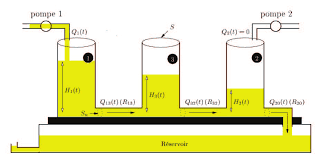
\includegraphics[width=12cm]{index.png}
   \captionof{figure}{\textit{Procédé trois bacs \cite{ref1}.}}
   \label{fig1}
 \end{center}   
   
   Depuis l’apparition de la nécessité de. \\
   
   Notre système est soumis à des perturbations exogènes suivants:
        
  \begin{enumerate}
      \item Un débit de fuite constante au niveau du bac numéro 1.
      \item Un bruit de mesure sur le capteur permettant la mesure de $h_{1}(t)$.
  \end{enumerate}
   
   Les systèmes .... bla bla... ajoutant à cela quelques problèmes connus:
    
   Malheureusement beaucoup d'entreprises ont bla bla. \\
   
   De nos jours....
   

%*********************** Performance et Robustesse **************
\chapter{Analyse d'une commande proportionnelle intégrale}

 \section{Le schéma bloc} 

	Après l'ajout du correcteur PI $K(p)=\frac {1+\tau_{i}p}{\tau_{i}p}$ à notre système, voici à quoi ressemble le       shéma bloc de l'asservissement:
% captures d’écrans 
  \begin{center}
    %
\includegraphics[scale=0.5]{Logo_UT3.jpg}
    \captionof{figure}{\textit{Schéma bloc de l'asservissement}}
    \label{fig2}
  \end{center}    
 
	On voit clairement que le signal du débit de fuite $W_{u}(p)$ du bac numéro 1 est relié au signal de commande $U(p)$ et le signal du bruit de mesure $b(p)$ et relié au signal de sortie $h_{1}(p)$.    
	
 \section{La validité de L'hypothèse} 
        
	Vu que l'eau est un liquide incompréssible, notre supposition du débit de fuite constant tient la route.
	
 \section{Le diagramme asymptotique de $K(p)=\frac {1+\tau_{i}p}{\tau_{i}p}$} 
 
 % captures d’écrans 
  \begin{center}
    %
\includegraphics[scale=0.5]{Logo_UT3.jpg}
    \captionof{figure}{\textit{Diagramme de Bode (gain et phase) }}
    \label{fig3}
  \end{center}

  \textbf{Nota:} Le correcteur a une allure d'un filtre passe bas.

 \section{Les spécifications satisfaites}
 
  \begin{itemize} [label=\ding{70},font=\small \color{black}]
  	\item Sans connaître les valeurs numérique du gain $k$ ou celle de la constante de temps $\tau_{i}$ utilisées dans le correcteur $K(p)$, on pourra déjà satisfaire la spécification $(b)$ car un integrateur $\frac{1}{p}$ ce que contient notre correcteur élimine l'erreur de position.
    \item à toi de jouer...
  \end{itemize}
 
 \section{Détermination de la contrainte sur le gabarit de $S(p)$}  
 
  \subsection{Création du gabarit de l'erreur de position}
  
  
  
  \subsection{Création du gabarit de l'erreur de vitesse}
  
 La figure au-dessus a ... bla bla ....\\
 
 Les bla bla ....\\
 
 Néanmoins, cette structure n’est jamais stable au fil du temps, ... bla bla.\\
  
 En court, il y a une différence entre ... bla bla ..., est fort envisageable qu’elle subira des changements dans le temps.
 
 \paragraph{Définition:}
  Bla bla ....

 \section{Section une}
  ggggggggggggggg
  \subsection{jamal}

%*********************** CONCLUSION **************
\chapter*{Conclusion}
 \addcontentsline{toc}{chapter}{Conclusion}
 
%*********************** Bibliographie ************ 
\bibliographystyle{alpha}
\bibliography{bibliographieperfoRobu}  

\end{document}\grid

